\documentclass{beamer}
\usepackage[utf8]{inputenc}
\usepackage{graphicx}
\usepackage{amsmath}
\usepackage{booktabs}
\usepackage{array}
\usepackage{booktabs}
\usepackage{multirow}
\usepackage{tabularx}
\usepackage[table]{xcolor}  % for coloring cells or rows
\usepackage{makecell}       % for multi-line cells

%\usetheme{CambridgeUS} % Neutral academic theme

\title[BOSS: Optimizing Shuttling]{BOSS: Blocking Algorithm for Optimizing Shuttling Scheduling in Ion Trap}
\author{Xian Wu, Chenghong Zhu, Jingbo Wang, Xin Wang}
\institute{HKUST (GZ) and BAQIS}
\date{\today}

\begin{document}
	
	\begin{frame}
		\titlepage
	\end{frame}
	
	\begin{frame}{Introduction: Ion Traps and Shuttling}
		\begin{itemize}
			\item Ion traps offer high-fidelity gates, long coherence, and full connectivity.
			\item Scalability is limited by heating and control complexity with more ions.
			\item Shuttling ions using microelectrodes allows fixed-laser execution zones.
			\item Reducing shuttle operations is key to fidelity and runtime.
		\end{itemize}
	\end{frame}
	
	\begin{frame}{Background: TILT Architecture}
		\begin{figure}
			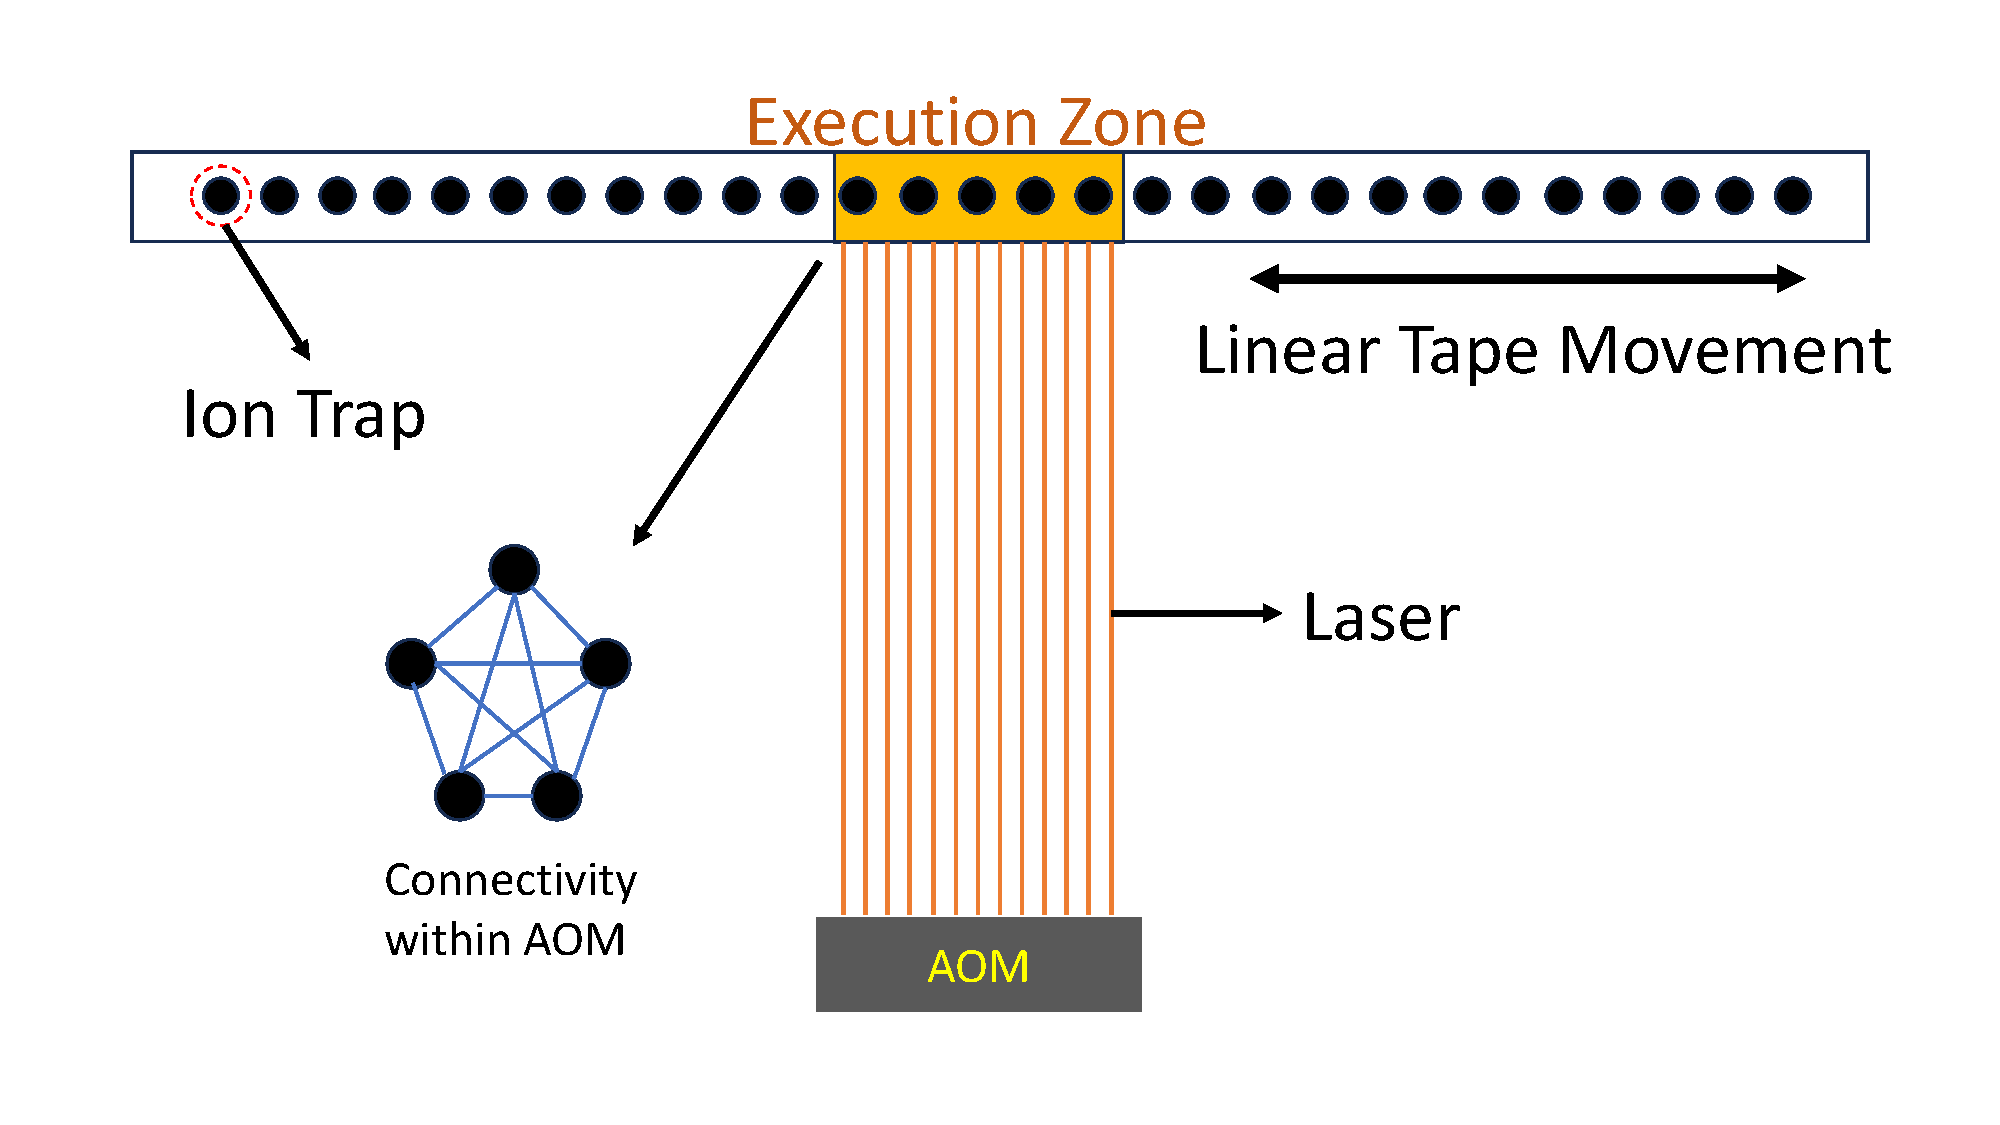
\includegraphics[width=.8\textwidth]{figure/TILT_laser.pdf}
			\caption[]{Linear trapped-ion quantum computer with full connectivity inside the AOM zone. Outside the zone, operations require ion shuttling. In TILT, each shuttle enables arbitrary-distance tape movement.}
		\end{figure}
	\end{frame}
	
	\begin{frame}{Background: Another Similar Architecture}
		\begin{figure}
			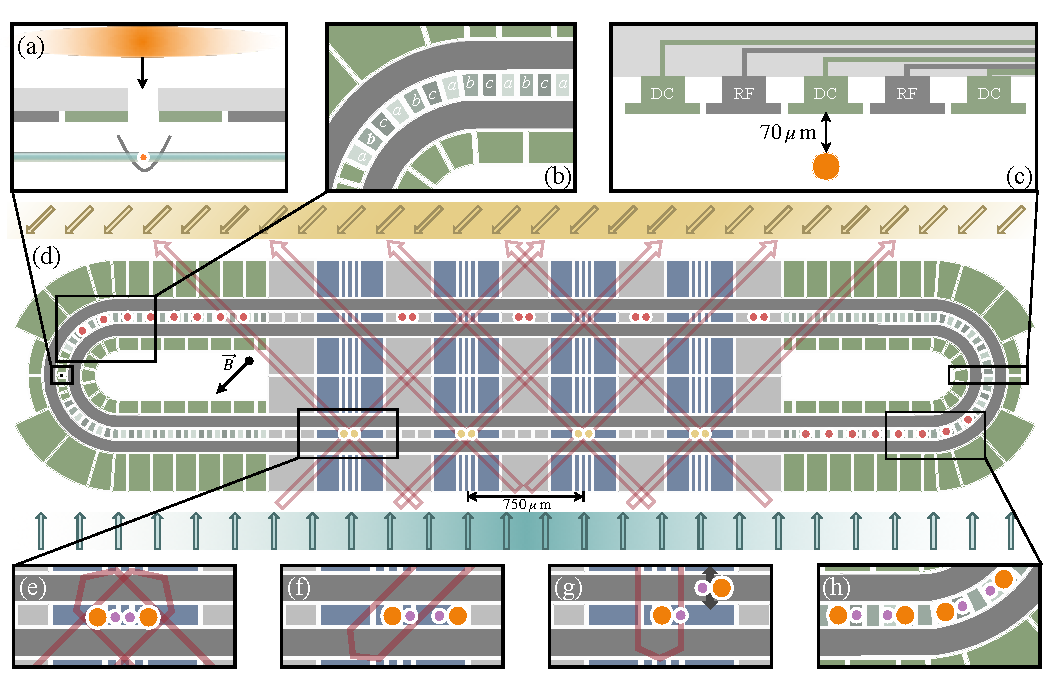
\includegraphics[width=.8\textwidth]{figure/h2_benchmarking_figure.pdf}
			\caption[]{An overview of the H2 ion trap designed by Quantinuum}
		\end{figure}
	\end{frame}
	
	\begin{frame}{Motivation: Optimize Shuttling}
		\begin{itemize}
			\item Prior compilers insert SWAPs heuristically without minimizing shuttles.
			\item Excessive shuttles lead to fidelity loss and longer circuit runtime.
			\item Opportunity: Use ion trap full connectivity in fixed zones efficiently.
			\item Need for a better compilation strategy tailored to TILT architecture.
		\end{itemize}
	\end{frame}
	
	\begin{frame}{Methods: BOSS Workflow Overview}
		\begin{figure}
			\centering
			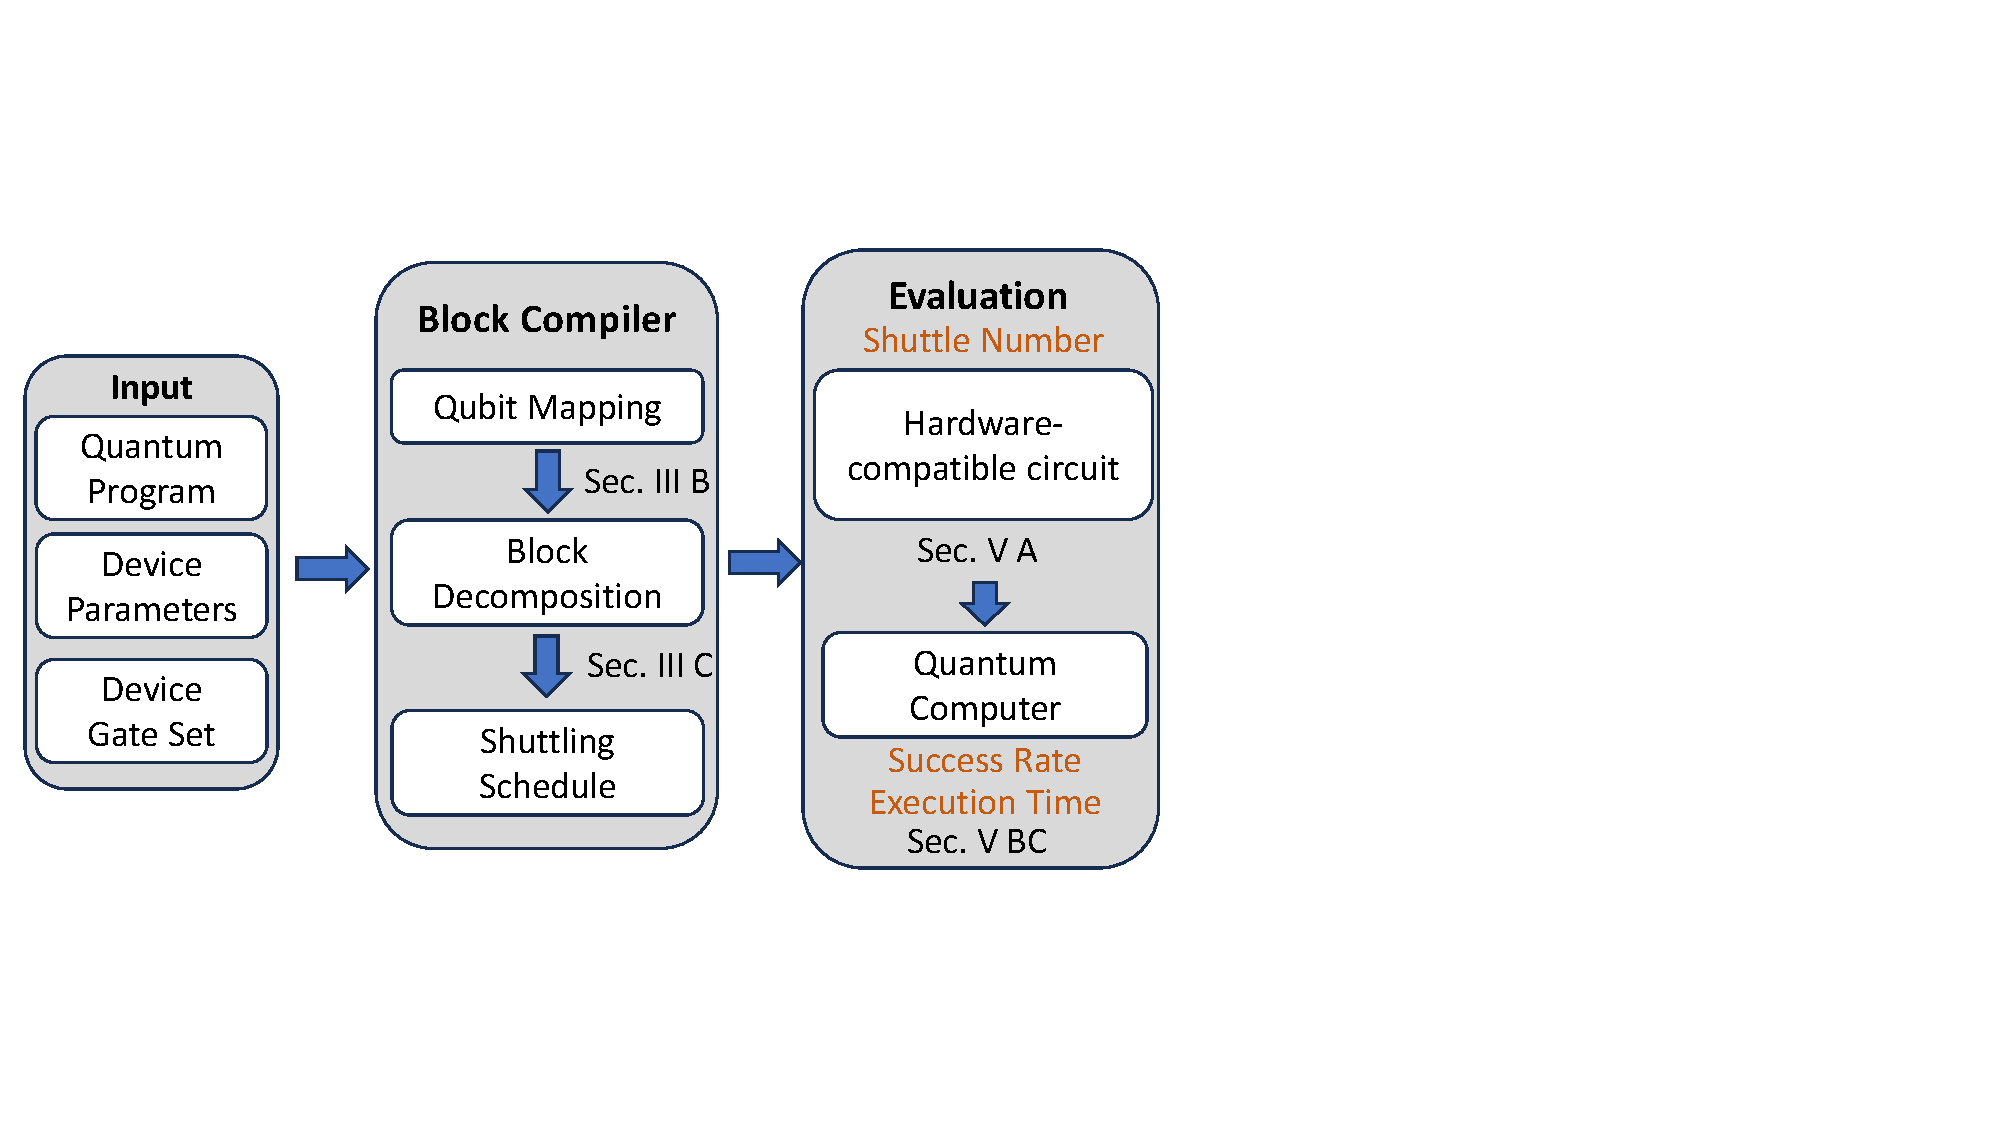
\includegraphics[width=0.85\textwidth]{figure/TILT_overview.pdf}
			\caption{Inputs: Quantum circuit, hardware specs, native gates. Outputs: Compiled schedule with minimized shuttle operations.}
		\end{figure}
	\end{frame}
	
	\begin{frame}{Methods: Circuit Blocking}
		\begin{figure}
			\centering
			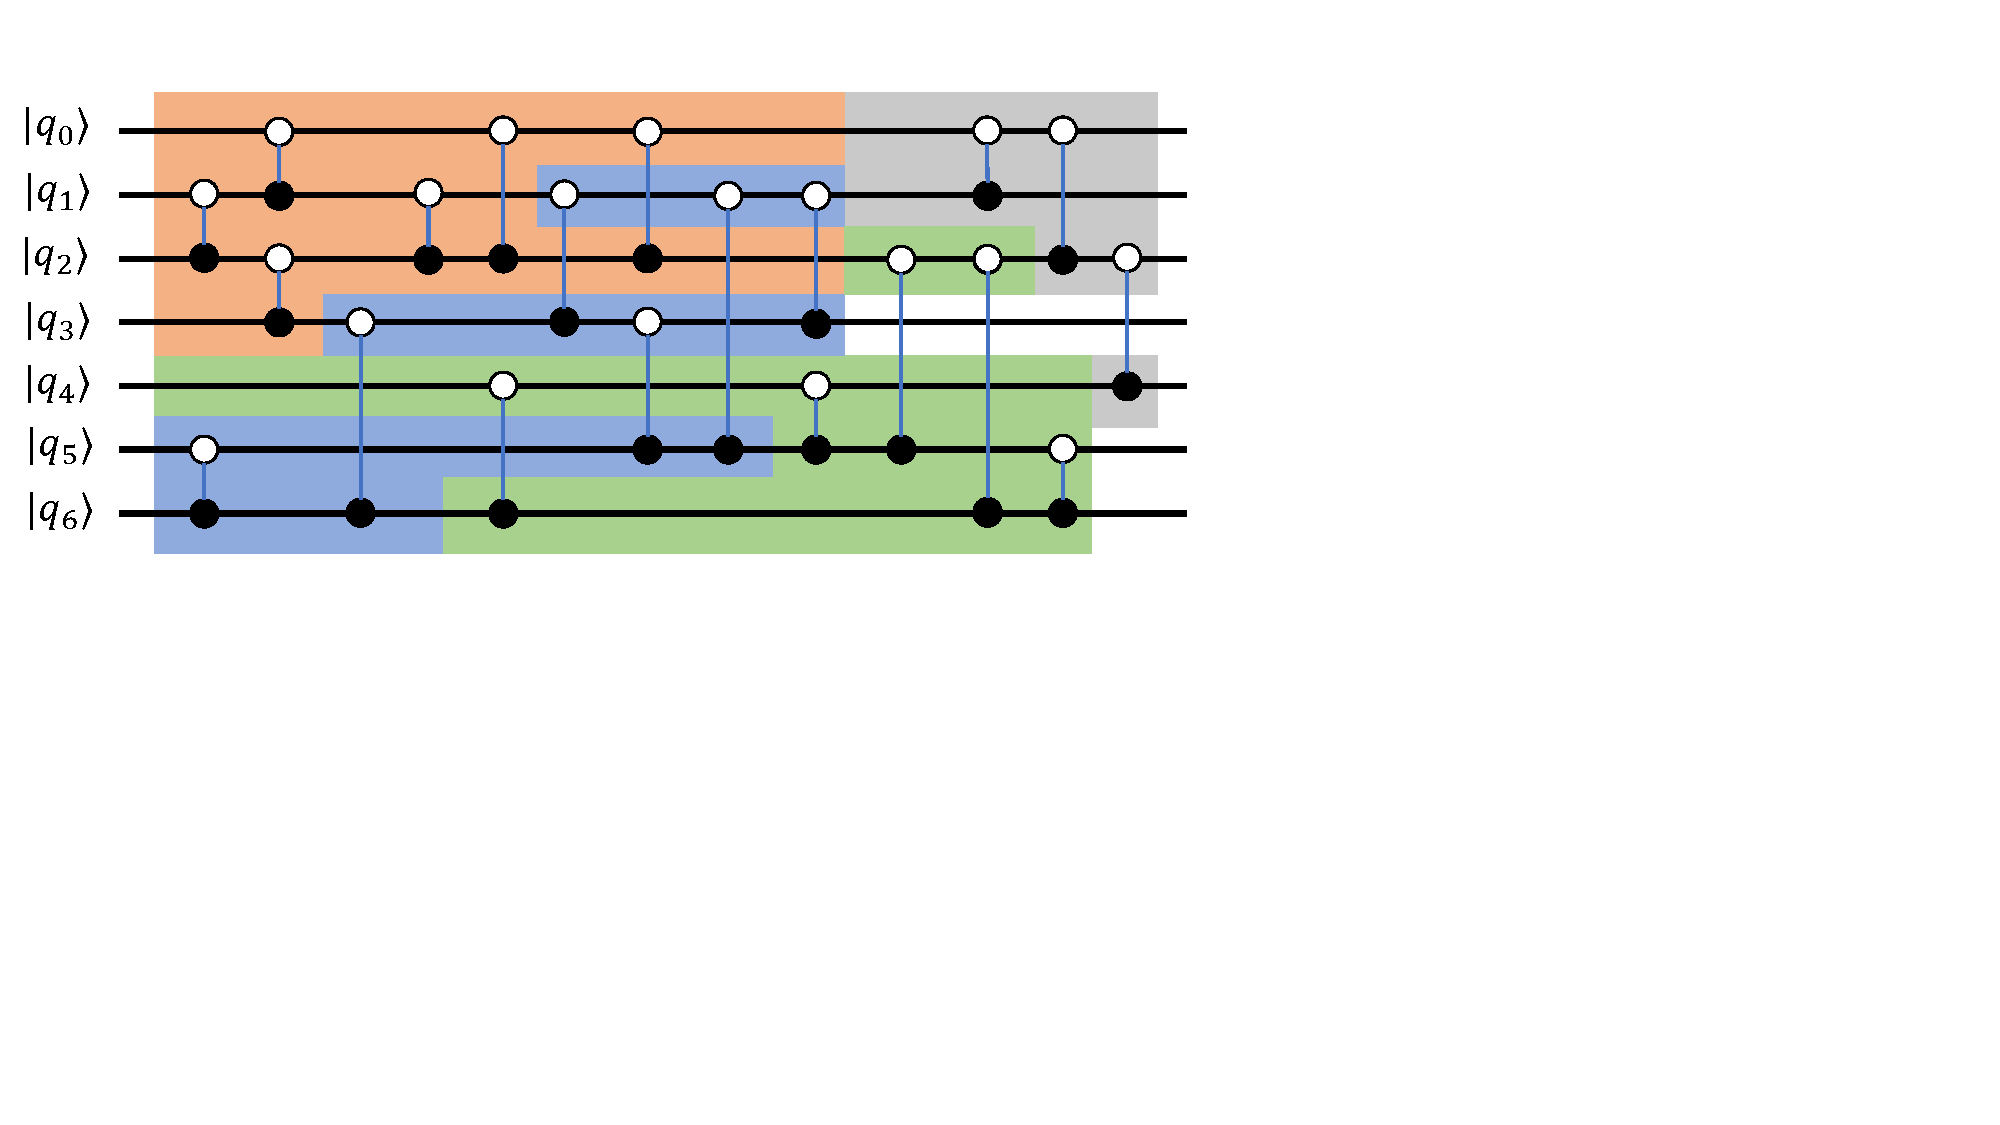
\includegraphics[width=0.8\textwidth]{figure/circuit-blocking.pdf}
			\caption{An example of circuit blocking, the maximal block size is 4. Gates are grouped into blocks respecting the AOM zone size. More gates per block $\Rightarrow$ fewer shuttles.}
		\end{figure}
	\end{frame}
	
	\begin{frame}{Methods: Block Scheduling Strategy}
		\begin{figure}
			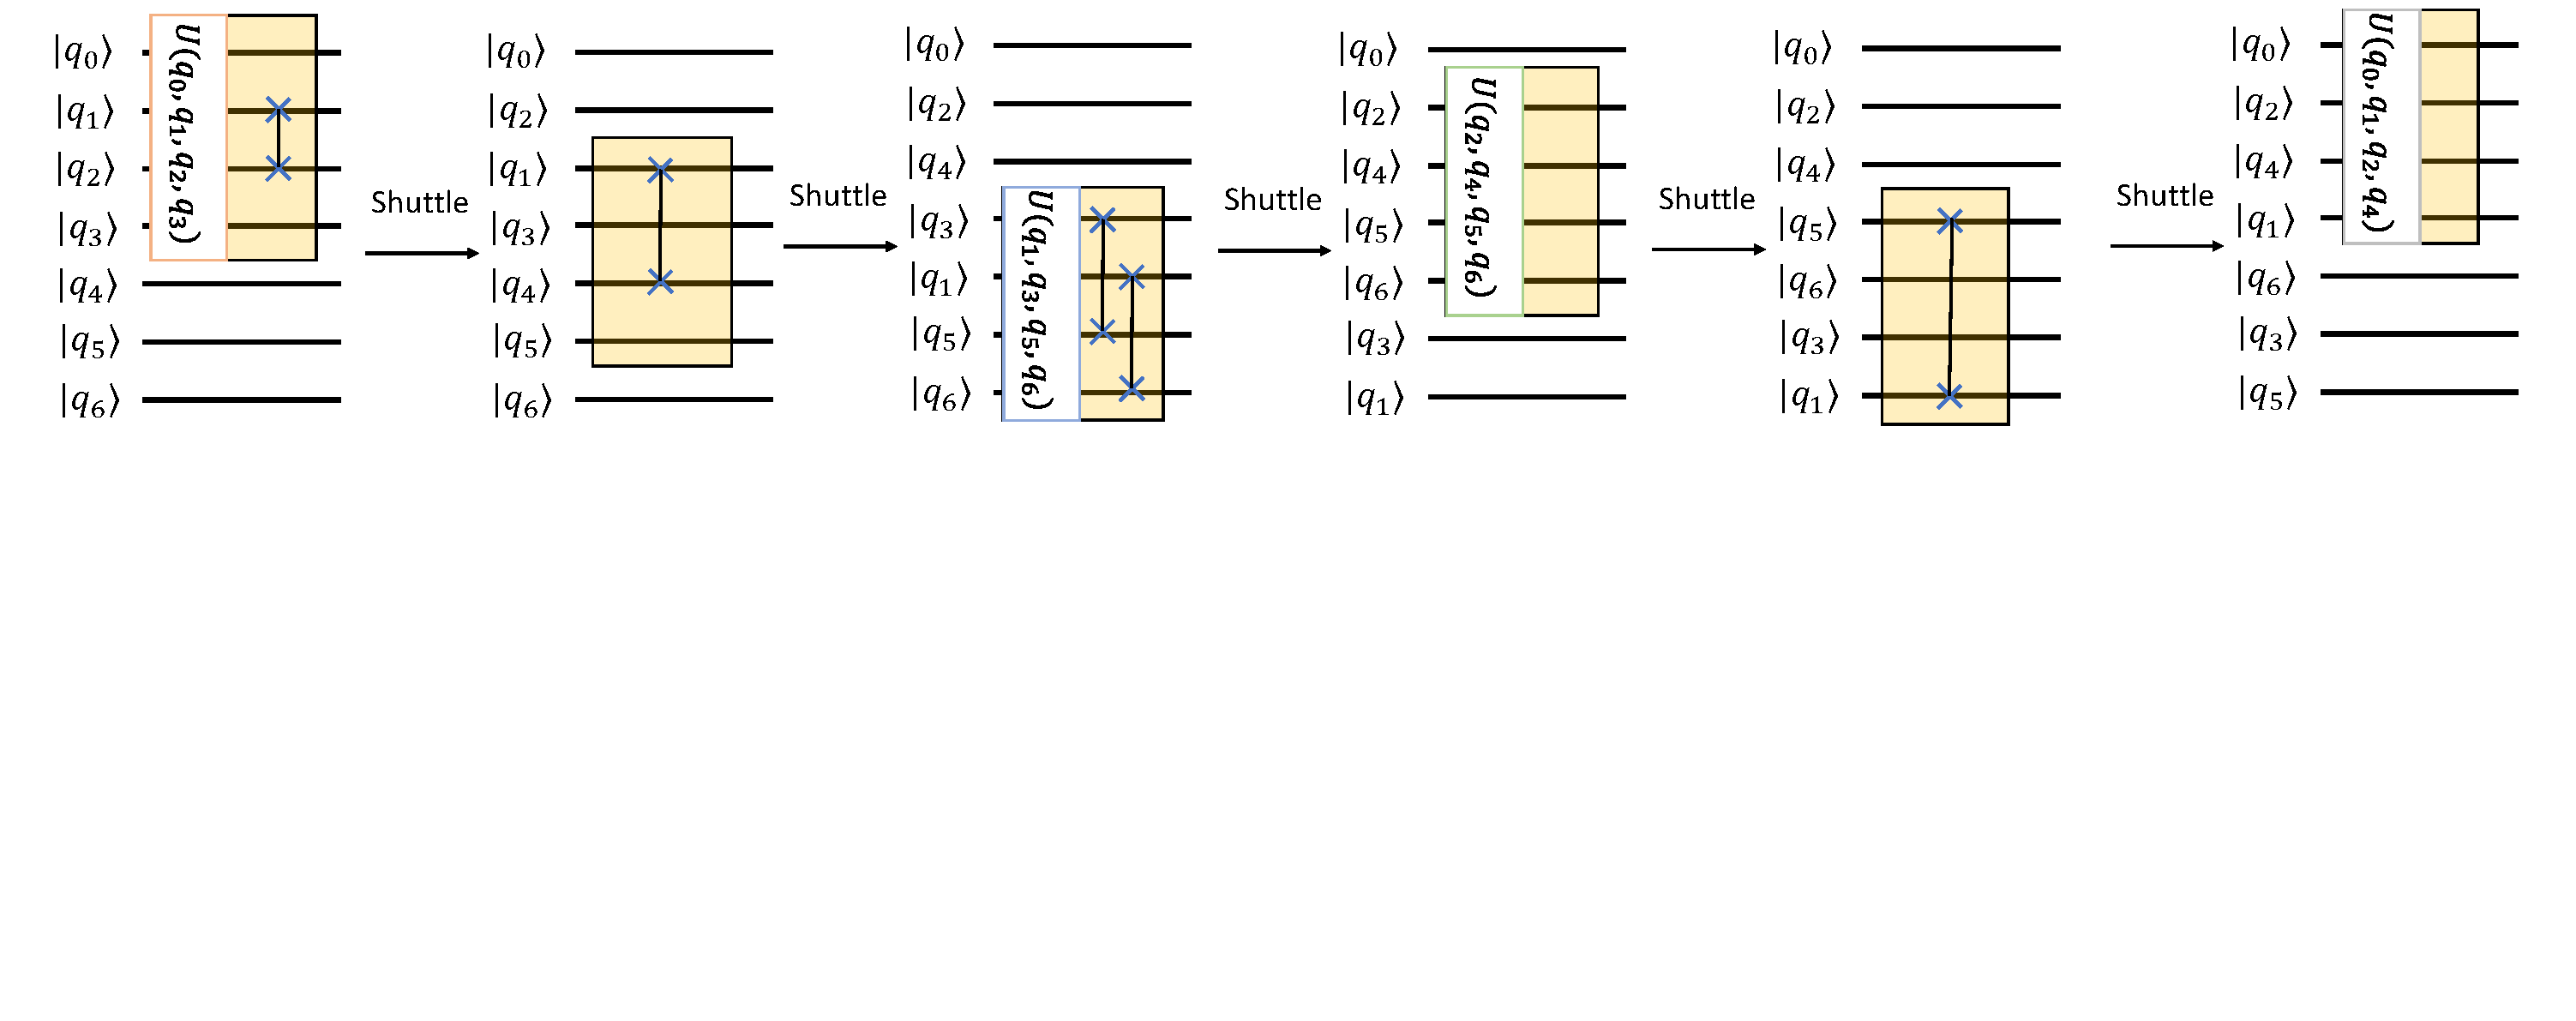
\includegraphics[width=.9\textwidth]{figure/block-schedule-long.pdf}
			\caption[]{Example of block scheduling: a block executes when all required qubits are in the execution zone; otherwise, shuttling and SWAP gates are used to gather them.}
		\end{figure}
	\end{frame}
	
	\begin{frame}{Overall Results}
%		\begin{figure}
%			\centering
%			\includegraphics[width=0.7\textwidth]{figure/different-implement-16.pdf}
%			\caption{Up to 96.1\% fewer shuttles (SQRT), 16.6\% average reduction.}
%		\end{figure}
		\begin{table}[b]
			\centering
				\resizebox{\textwidth}{!}{
					\begin{tabular}{|c|c|c|c|c|c|c|c|c|c|c|c|}
					\hline
					\textbf{Application} & \textbf{AOM size}
					& $T_{pre}(s)$ & $T_{boss}(s)$&$S_{base}$& $S_{pre}$ & $S_{boss}$ & $\Delta S$ & $\Delta S/S_{pre}$ 
					&$t_{pre}(s)$ &$t_{boss}(s)$ &$t_{pre}/t_{boss}$ \\
					\hline
					\hline
					Adder&16 &6.216& 0.007&35& 10 & 8  & 2& 20\% 
					& 2.967 & 0.0378 & 78.6\\
					BV&16  &1.579&0.006 & 4 & 4& 4&0 & 0\% 
					&0.856& 0.0354 & 24.2\\
					QAOA&16  &2.761 &0.038 &113 & 18 & 18 &0 & 0\% 
					& 1.564 & 0.0418 & 37.4 \\
					ALT &16 &2.880&0.013 &91 &24& 20& 4 &16.7\% &1.311 &0.0256 &51.2\\
					RCS&16  & 3.149&0.045&277&65  & 106 &-41 & -63.1\% 
					&1.704 & 0.2057 & 8.3 \\
					QFT &16 &64.823& 0.064 &407 & 162 & 48  &114 & 70.4\%  
					& 24.820 & 0.4405 & 56.3\\
					SQRT&16  &131.245 & 0.430 & 816 & 168 & 71 &97  & 57.7\%  
					& 46.554 & 0.2593 & 179.6 \\
					\hline
					Adder&32&3.250&0.006 & 5 & 5& 4 &1 & 20\% 
					&3.252 & 0.0372 & 87.5 \\
					BV&32 &0.902& 0.005& 2& 2 & 2&0 & 0\% 
					&0.987 & 0.0527 & 18.7\\
					QAOA&32   &1.112&0.029 & 40 & 4&  4&0  & 0\%
					& 1.357 & 0.0284 & 47.7\\
					ALT &32&1.404&0.019 &38 &8 &5 &3& 37.5\% & 1.017  & 0.0178  & 57.1 \\
					RCS&32 &0.681&0.017 & 86 & 11 &  21&-10  & -90.9\% 
					&0.856 &0.1307 & 6.5\\
					QFT &32 &37.341& 0.051& 69 & 69& 8 & 61 & 88.4\% 
					& 33.876 & 0.3926 & 86.3\\
					SQRT&32  &56.309 & 0.013 & 431 & 76 & 3 & 73 & 96.1\%  
					& 40.817 & 0.2070 & 107.1\\
					\hline
				\end{tabular}}
			% }
		\caption{Comparison with prior work on compilation time, number of shuttle operations, and total execution time (lower is better). The method achieves up to a 96.1\% reduction in shuttling (SQRT benchmark) and an average reduction of 16.6\%.
		\textbf{$T$}: compilation time; \textbf{$S$}: shuttle number; \textbf{$t$}: execution time(Trout model).}
		\end{table}
	\end{frame}
	
	\begin{frame}{Results: Shuttle Number}
		\begin{figure}
			\centering
			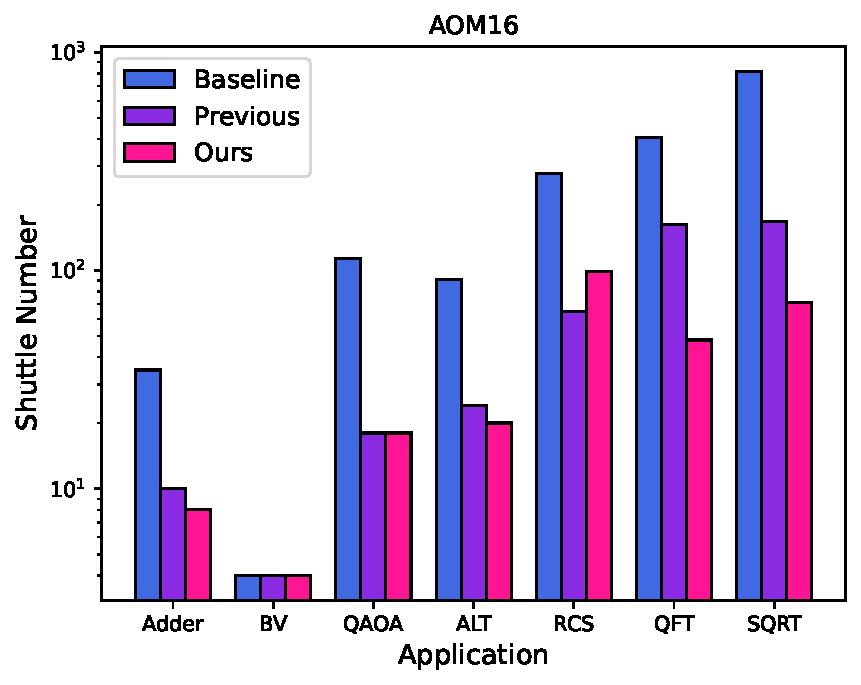
\includegraphics[width=0.7\textwidth]{figure/Shuttle-comparation.pdf}
			\caption{Number of shuttling operations.}
		\end{figure}
	\end{frame}
	
	\begin{frame}{Results: Fidelity}
		\begin{figure}
			\centering
			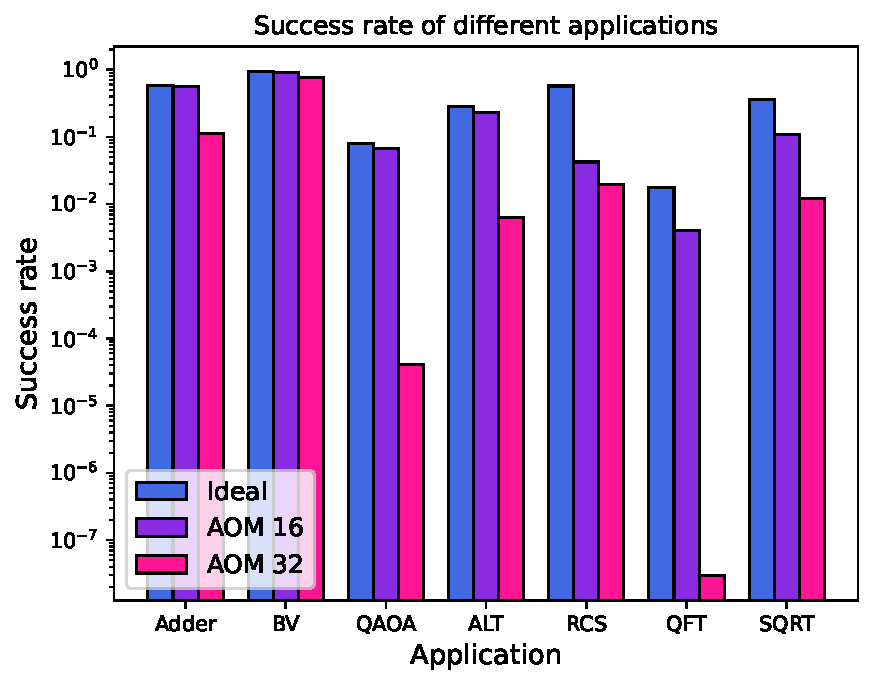
\includegraphics[width=0.7\textwidth]{figure/Fidelity-true.pdf}
			\caption{Orders-of-magnitude improvement in success rate due to fewer shuttles.}
		\end{figure}
	\end{frame}
	
	\begin{frame}{Results: Execution Time}
		\begin{figure}
			\centering
			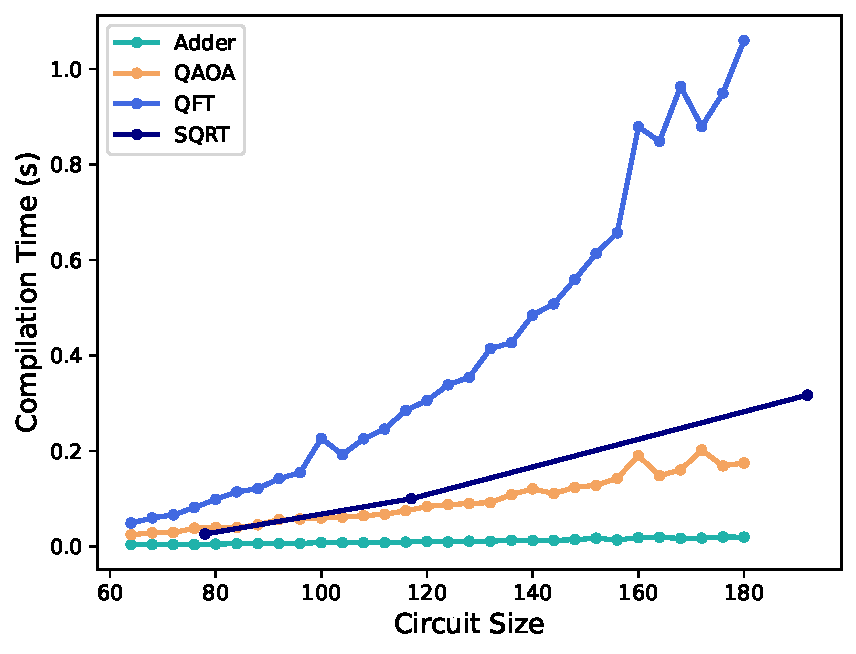
\includegraphics[width=0.7\textwidth]{figure/scalability1.pdf}
			\caption{The compilation time varies with the size of the circuit. The circuit size refers to the number of qubits in the circuit, and the AOM size is 16.}
		\end{figure}
	\end{frame}
	
	\section{Conclusion}
	\begin{frame}{Conclusion}
		\begin{itemize}
			\item BOSS reduces shuttling and improves fidelity and runtime.
			\item Efficient: Compiles large circuits ($>100$ qubits) in under 2s.
			\item Scalable and adaptable to future ion trap designs.
		\end{itemize}
	\end{frame}
	
\end{document}
